\documentclass[a4paper,twoside,12pt]{book}

\usepackage{calc}
\usepackage{setspace}
\usepackage{graphicx}
\usepackage{amsmath}
\usepackage{float}
\usepackage{todonotes}

%%%%%%% Clickable links %%%%%%%
\usepackage{hyperref}
\hypersetup{
	colorlinks,
	citecolor=black,
	filecolor=black,
	linkcolor=black,
	urlcolor=black
}

%%%%%%% Word Counting %%%%%%%
\newcommand{\detailtexcount}[1]{%
  \immediate\write18{texcount -merge -sum -q #1.tex output.bbl > #1.wcdetail }%
  \verbatiminput{#1.wcdetail}%
}
\newcommand{\quickwordcount}[1]{%
  \immediate\write18{texcount -1 -sum -merge -q #1.tex output.bbl > #1-words.sum }%
  \input{#1-words.sum} words%
}
\newcommand{\quickcharcount}[1]{%
  \immediate\write18{texcount -1 -sum -merge -char -q #1.tex output.bbl > #1-chars.sum }%
  \input{#1-chars.sum} characters (not including spaces)%
}


%%%%%%% Page styles %%%%%%%
\setlength{\hoffset}{-1in} \setlength{\oddsidemargin}{40mm} \setlength{\evensidemargin}{30mm}
\setlength{\textwidth}{\paperwidth-\oddsidemargin-\evensidemargin} \onehalfspacing

%%%%%%% Document starts here
\begin{document}

%%%%%%% Title Page %%%%%%%
\frontmatter
\begin{titlepage} \null\vfill \centering
  {\Huge \bf Quantifying the Impact of Atmospheric and Oceanic Processes on the behaviour of Sea Ice in Antarctica} \\ \vspace{20mm} {\Large Hamish Jelleyman} \\ \vspace{20mm} 
\includegraphics{Images/UoA_Crest.eps} \\ \vspace{20mm} A thesis submitted in fulfilment of the requirements \\ for the degree of Master of Science in Physics \\ \vspace{20mm} The University of Auckland \\ 2020
\vfill\null \end{titlepage}

\chapter*{Abstract}
\chapter*{Acknowledgements}

\tableofcontents
\listoffigures
\listoftables

%%%%%%% Main text %%%%%%%
\mainmatter
\chapter{Introductions}
This is all the preliminary sections of the thesis. We will introduce the project and the key ideas surrounding the project. We will include a rigorous literature review which explores papers relevant to this project and the surrounding research. We also discuss the different related datasets which we either use or consider using.
\pagebreak
\section{Introduction}
This is the place where we loosely introduce and motivate the project which we will do this year. We will summarise (in short) the rest of the report here.
\pagebreak
\section{Literature Review}
In this literature review, we aim to tell you a story of research which has been done in this area of research before this point in time. In doing this we hope to provide the reader of this thesis an understanding of the strengths and weaknesses of relevant literature. What has and what hasn't been done by other researchers. We also will take some time to delve into the papers most relevant to this project by discussing methods and results which we at least considered using in the process of doing our research.\medskip

This literature review will be structured to look at specific topics which are somehow related to the research we carried out. These topics are included in the left hand column of the table below, alongside with the counts for the numbers of papers we looked at for each topic.

\begin{table}[H]
\resizebox{\textwidth}{!}{%
\begin{tabular}{@{}r|r|c@{}}
\toprule
\multicolumn{2}{r|}{\textbf{Topic/Source}}                                          & \textbf{Number of Papers} \\ \midrule
\multicolumn{2}{r|}{From Honors}                                                    & 25                        \\
\multicolumn{2}{r|}{Sea ice trends and variability in Antarctica}                   &                           \\
\multicolumn{2}{r|}{Atmospheric trends and variability in Antarctica}               &                           \\
\multicolumn{2}{r|}{Oceanic trends and variability in Antarctica}                   &                           \\
\multicolumn{2}{r|}{Sea ice and the atmosphere}                                     &                           \\
\multicolumn{2}{r|}{Sea ice and the ocean}                                          &                           \\
\multirow{3}{*}{Comparing different weather datasets} & Methods of correlation      &                           \\
                                                      & Useful measures             &                           \\
                                                      & Ways of thinking about this &                           \\ \bottomrule
\end{tabular}}
\caption{WIP: Topics covered by different papers}
\end{table}

\subsection{Sea ice trends and variability in Antarctica}
This section of the literature review will discuss the research papers which we looked at regarding the trends and variability of sea ice extent and area around Antarctica.
\subsection{Atmospheric trends and variability in Antarctica}
This section of the literature review will discuss the research papers which we looked at regarding the trends and variability of atmospheric conditions around Antarctica.
\subsection{Oceanic trends and variability in Antarctica}
This section of the literature review will discuss the research papers which we looked at regarding the trends and variability of oceanic conditions around Antarctica.
\subsection{Sea ice and atmospheric processes}
This section of the literature review will discuss in some detail, the research which has been carried out to investigate the relationship between sea ice and atmospheric processes in Antarctica and globally.
\subsection{Sea ice and oceanic processes}
This section of the literature review will discuss in some detail, the research which has been carried out to investigate the relationship between sea ice and oceanic processes in Antarctica and globally.
\subsection{Statistical Methods}
This section of the literature review will cover a number of the statistical methods used in different papers which we looked at using for this project. 
\medskip

One such technique we may want to use is change-point analysis as discussed by Beaulieu, Chen, and Sarminento \cite{Beaulieu2012}.
This is used for looking at changes in temporal regimes for time series, they propose it for the purposes of detecting abrupt climate variations. We will also use it for this purpose. The paper provides a good overview of different types of change-points which exist  \textcolor{red}{Include figure?} and a good overview of different ways in which people go about detecting them. They set out to describe and extend an informational approach to this problem, making use of the Schwartz information criterion to identify change points for a variety of fitting models.
\pagebreak
\section{Data}
This will be a summary of the data we use in this project and some data which we don't (but is used by other researchers)
How is it collected? What format is it in?
How reliable is it?
\chapter{Methods}
\label{Chap:Methods}

\section{Introduction to Methods}
This chapter includes a description of the methods employed in this project. We will cover everything from standardising the datasets for easy comparison through to \todo{finish this once the section is done}

\section{Regridding Data}
Because we use a variety of datasets which come in a variety of structures, it is important that standardise the spatial dimensions of each data source. One way we do this is by interpolating each dataset to have a consistent spatial arrangement. This allows for better quality results and makes it easier to calculate measures such as the correlation between 2m temperature and sea ice concentration.

We do the interpolation using the python package Scipy, which makes use of a piecewise cubic, continuously differentiable (C1), and approximately curvature-minimizing polynomial surface to determine the value of our given variable at a chosen location. \todo{cite this or something?}

We converted the temperature data to the projection the sea ice data is provided in; a south polar stereographic projection with regular grid cells of 25km$\times$25km. We found this resolution to have a good balance between reasonable runtimes and good quality results.


\section{Pearson Correlation Coefficient}
\label{Methods:pearson}
\todo{Do we need a citation for this?}
One comparison which we used for identifying connections between two different time series or different time series components is the Pearson correlation component. Taking a time series $x$, and a time series $y$, with elements $x_i$ and $y_i$, and means denoted by $\bar{x}$ and $\bar{y}$; we can calculate the Pearson correlation coefficient $r_{xy}$.

\begin{equation}
\label{eq:pearson}
    r(x, y)=\frac{\sum_{i=1}^{n}\left(x_{i}-\overline{x}\right)\left(y_{i}-\overline{y}\right)}{\sqrt{\sum_{i=1}^{n}\left(x_{i}-\overline{x}\right)^{2}} \sqrt{\sum_{i=1}^{n}\left(y_{i}-\overline{y}\right)^{2}}}
\end{equation}

\chapter{Results and Discussion}
\label{Chap:Results}

\section{Introduction to Results and Discussion}
In this chapter we will present our results for this project and discuss their significance and shortcomings.\todo{finish this}

\section{Air Temperature and SIC Correlations}
\begin{figure}[H]
    \centering
    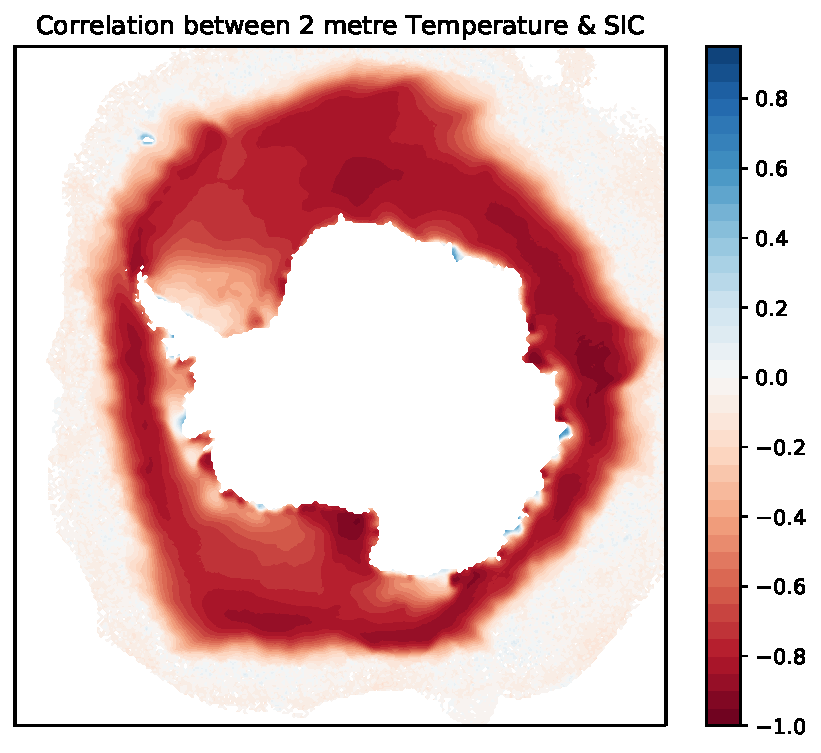
\includegraphics{Images/tempcorrwithsic.pdf}
    \caption{Correlation between temperature at 2m with sea ice concentration.}
    \label{fig:results:2mtemp_corr_with_sic}
\end{figure}
Above we have the correlation between 2 metre air temperature and sea ice concentration over Antarctica. The result that the temperature is negatively correlated with the concentration of sea ice in Antarctica is hardly surprising. Higher temperatures will be associated in the melting of ice. This both intuitively makes sense and is supported by the first law of thermodynamics (Conservation of energy). The main feature of interest in this plot is the regions which are close to the pole and there are lower correlations between 2m-temperature and SIC. It is possible that this is due to low variability in SIC in these regions over the entirety of each year.

%%%%%%% Bibliography %%%%%%%
\bibliographystyle{Unsrtrjk}
\bibliography{references}
% Don't count these!

\chapter{Word Counts}
\quickwordcount{main}
% \detailtexcount{main}


\end{document} 